\subsection{Mikro DC Motor 6V -- Sumber Rotasi Penggerak Kipas}
\label{subsec:dc_motor_6v}

% ---------------------------------------------------------------------
\subsubsection{Identitas dan Fungsi}
\begin{wrapfigure}{r}{0.3\textwidth}
	\vspace{-45pt}
	\centering
	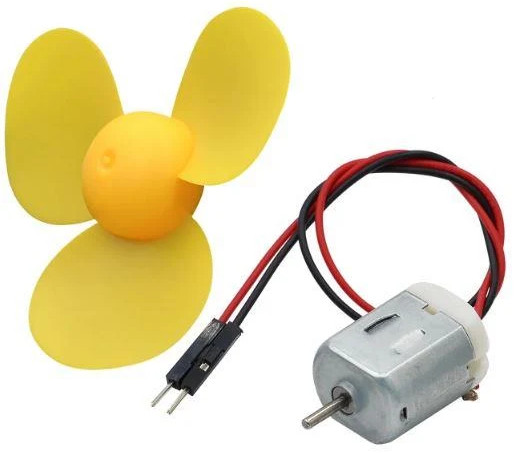
\includegraphics[width=\linewidth]{images/dc_motor_fan.jpg}
	\caption{Mikro DC motor 6V dengan baling-baling kipas.}
	\label{fig:dc_motor_front}
\end{wrapfigure}

Mikro DC Motor 6V (tipe FAFC-130SAV-14150) adalah sebuah aktuator putar kontinu yang mengonversi energi listrik arus searah menjadi energi mekanis berupa putaran poros. Dalam sistem ini, motor berfungsi sebagai penggerak utama baling-baling kipas sirkulasi udara. Komponen ini memiliki tegangan kerja nominal $6{,}0\,\text{V DC}$ dengan rentang operasional $4{,}5\text{--}7{,}5\,\text{V DC}$. Motor mampu memberikan kecepatan rotasi tinggi mencapai $12.400\,\text{RPM}$ pada kondisi tanpa beban serta $9.601\,\text{RPM}$ pada beban kerja pengenal ($13{,}5\,\text{g}\cdot\text{cm}$). Dengan dimensi bodi yang ringkas ($25{,}0 \times 20{,}1 \times 15{,}1\,\text{mm}$), ukuran poros berdiameter $2{,}0\,\text{mm}$ dengan panjang $8{,}5\,\text{mm}$, serta bobot ringan $\approx 17\,\text{gram}$, aktuator ini sangat ideal diintegrasikan sebagai modul pendingin sirkulasi udara.

\begin{table}[H]
	\centering
	\caption{Identitas komponen Mikro DC Motor 6V}
	\label{tab:dc_motor_identitas}
	\small
	\begin{tabularx}{\textwidth}{@{} p{3.8cm} X @{}}
		\toprule
		Parameter          & Keterangan                                                                      \\
		\midrule
		Nama komponen      & Mikro DC Motor 6V (Dinamo Penggerak Kipas)                                      \\
		Model/part number  & FAFC-130SAV-14150 (FONEACC CO., LIMITED)                                        \\
		Jenis              & Aktuator Elektromekanis / Motor Arus Searah Bersikat (\textit{Brushed DC})      \\
		Fungsi utama       & Mengonversi tegangan/arus DC menjadi energi rotasi mekanis memutar baling kipas \\
		Sumber dokumentasi & FAFC-130 Micro Brush DC Electric Motor Datasheet (FONEACC)                      \\
		\bottomrule
	\end{tabularx}
\end{table}

% ---------------------------------------------------------------------
\subsubsection{Prinsip Kerja}
Cara kerja mikro DC motor didasarkan pada \textbf{Gaya Lorentz} dan \textbf{induksi elektromagnetik}. Di dalam rumah motor (\textit{stator}), terdapat dua elemen utama yang saling berinteraksi secara fisika:

\begin{enumerate}
	\item \textbf{Bagian Stator dan Rotor (Magnet Permanen \& Kumparan Jangkar):}
	      Dinding bagian dalam rumah motor dilengkapi magnet permanen yang menghasilkan medan magnet tetap ($B$). Sementara itu, bagian poros utama (\textit{rotor}) memuat gulungan kawat tembaga (kumparan) yang terhubung ke komutator. Ketika arus listrik ($I$) dialirkan melewati gulungan kawat yang berada di dalam medan magnet tersebut, timbul Gaya Lorentz mekanis ($F$) yang mendorong kumparan dan memaksa poros motor untuk berputar.

	\item \textbf{Bagian Pengalihan Arus Mekanis (Komutator \& Sikat Tembaga):}
	      Agar poros motor dapat terus berputar ke satu arah yang sama, komutator tembaga bersama \textit{brushes} secara mekanis membalik arah aliran arus pada kumparan setiap kali \textit{rotor} melewati kutub magnetik. Sementara itu, untuk mengendalikan kecepatan putaran kipas secara halus melalui mikrokontroler, sirkuit \textit{driver} eksternal menggunakan \textit{Pulse Width Modulation} (PWM) untuk mengatur rata-rata tegangan yang disalurkan ke motor.
\end{enumerate}

\begin{figure}[H]
	\centering
	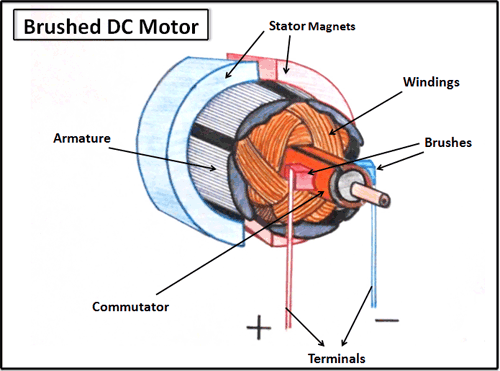
\includegraphics[width=0.55\textwidth]{images/dc_motor_internal.png}
	\caption{Struktur internal motor DC bersikat.}
	\label{fig:dc_motor_karakteristik}
\end{figure}

\paragraph{Konsep dan Formulasi Matematis Terkait}
Besar Gaya Lorentz $F$ yang bekerja pada kawat kumparan penghantar berpanjang $L$ di dalam medan magnet $B$ dirumuskan sebagai:

\begin{equation}
	F = I \cdot L \cdot B \cdot \sin(\alpha)
	\label{eq:dc_motor_lorentz}
\end{equation}

Sementara itu, hubungan antara tegangan masukan $V_{\text{in}}$, Gaya Gerak Listrik Balik (\textit{Back-EMF}) $E_b$, dan kecepatan sudut rotasi poros $\omega$ memenuhi persamaan:

\begin{equation}
	V_{\text{in}} = E_b + (I \cdot R_a) = (K_e \cdot \omega) + (I \cdot R_a)
	\label{eq:dc_motor_voltage}
\end{equation}

\noindent di mana:
\begin{itemize}
	\item $F$ = Gaya Lorentz penggerak rotasi ($\text{N}$).
	\item $I$ = Arus listrik jangkar yang mengalir melalui motor ($\text{A}$).
	\item $L$ = Panjang kawat tembaga di dalam medan magnet ($\text{m}$).
	\item $B$ = Rapat fluks medan magnet permanen ($\text{T}$).
	\item $V_{\text{in}}$ = Tegangan rata-rata masukan motor ($\text{V}$).
	\item $E_b$ = Tegangan induksi balik / \textit{Back-EMF} ($\text{V}$).
	\item $K_e$ = Konstanta kelektrisan motor ($\text{V}\cdot\text{s/rad}$).
	\item $\omega$ = Kecepatan rotasi poros motor ($\text{rad/s}$).
	\item $R_a$ = Resistansi dalam kumparan jangkar ($\Omega$).
\end{itemize}

% ---------------------------------------------------------------------
\subsubsection{Alur Kerja Internal dan Protokol Komunikasi}
Alur pemrosesan operasional motor DC mengikuti pola \textbf{Input $\rightarrow$ Proses $\rightarrow$ Output}. Pin GPIO mikrokontroler \textbf{tidak dihubungkan secara langsung} ke terminal DC motor karena keterbatasan batas arus pin GPIO ($\le 40\,\text{mA}$) serta risiko kerusakan akibat lonjakan arus pemicuan awal dan arus macet (\textit{stall current}) yang dapat mencapai $2{,}0\,\text{A}$. Oleh karena itu, pin GPIO hanya bertindak sebagai pengirim sinyal pemicu ke modul perantara (\textit{driver}/relai):

\begin{enumerate}
	\item \textbf{Input:} Penerimaan sinyal kontrol PWM atau sinyal diskret biner (LOW/HIGH) dari pin GPIO mikrokontroler menuju modul sakelar penggerak daya eksternal (\textit{relay board} atau \textit{transistor/MOSFET driver}).
	\item \textbf{Proses:} Modul penggerak daya mengisolasi dan menyalurkan arus dari catu daya utama $6{,}0\,\text{V DC}$ ke terminal motor, memicu pembentukan medan elektromagnetik pada \textit{rotor} yang berinteraksi dengan magnet permanen \textit{stator}.
	\item \textbf{Output:} Putaran mekanis poros motor yang memutar baling-baling kipas untuk menghasilkan hembusan aliran udara.
\end{enumerate}

\paragraph{Detail Sinyal Kontrol PWM}
Mikro DC motor beroperasi berdasarkan tegangan rata-rata yang disalurkan melalui sirkuit \textit{driver} eksternal. Pin GPIO mikrokontroler mengirimkan sinyal kontrol PWM berlevel logika $5\,\text{V}$ TTL sebagai sinyal pemicu. Sinyal pemicu ini memerintahkan sirkuit \textit{driver} untuk memberikan tegangan daya $6{,}0\,\text{V DC}$ dari catu daya eksternal menuju terminal motor secara sefase:

\begin{itemize}
	\item \textbf{Siklus Kerja 0\% (\textit{Duty Cycle} 0\%):} Sinyal GPIO $0\,\text{V}$ mematikan sakelar \textit{driver}, tegangan efektif pada motor $0\,\text{V DC}$ ($0\,\text{RPM}$).
	\item \textbf{Siklus Kerja 50\% (\textit{Duty Cycle} 50\%):} Pulsa GPIO $5\,\text{V}$ mengaktifkan \textit{driver} selama setengah periode, menghasilkan tegangan rata-rata $\approx 3\,\text{V DC}$ pada motor ($\approx 50\%$ RPM nominal).
	\item \textbf{Siklus Kerja 100\% (\textit{Duty Cycle} 100\%):} Sinyal GPIO HIGH ($5\,\text{V}$) secara jenuh mengaktifkan \textit{driver}, memberikan tegangan penuh $6{,}0\,\text{V DC}$ pada motor ($100\%$ RPM nominal).
\end{itemize}

\begin{figure}[htbp]
	\centering
	\begin{tikzpicture}[x=0.22mm, y=10mm, >=Stealth, font=\sffamily\small]
		% Axis Utama
		\draw[->, color=gray!60, thick] (0, 0) -- (480, 0) node[right, color=black] {\textit{t}};
		\draw[->, color=gray!60, thick] (0, 0) -- (0, 3.3) node[above=2pt, color=black] {V};

		% Level Tegangan Sumbu Y
		\node[left=4pt, font=\scriptsize, color=blue!80!black, align=right] at (0, 2.0) {\shortstack[r]{\textbf{6\,V}\\\textit{(Daya Motor)}}};
		\node[left=4pt, font=\scriptsize, color=teal!80!black, align=right] at (0, 1.3) {\shortstack[r]{\textbf{5\,V}\\\textit{(Sinyal GPIO)}}};
		\node[left=4pt, font=\scriptsize, align=right] at (0, 0.3) {\shortstack[r]{\textbf{0\,V}\\\textit{(LOW / OFF)}}};

		% Garis Acuan Putus-Putus
		\draw[dotted, color=blue!30] (0, 2.0) -- (450, 2.0);
		\draw[dotted, color=teal!30] (0, 1.3) -- (450, 1.3);
		\draw[dotted, color=gray!40] (0, 0.3) -- (450, 0.3);

		% PERIODE 1: Duty Cycle 25%
		\draw[thick, color=teal!80!black] (0, 0.3) -- (30, 0.3);
		\draw[ultra thick, color={rgb,255:red,30;green,64;blue,175}] (0, 0.3) -- (30, 0.3);
		\draw[thick, color=teal!80!black] (30, 0.3) -- (30, 1.3) -- (55, 1.3) -- (55, 0.3) -- (130, 0.3);
		\draw[ultra thick, color={rgb,255:red,30;green,64;blue,175}] (30, 0.3) -- (30, 2.0) -- (55, 2.0) -- (55, 0.3) -- (130, 0.3);

		% PERIODE 2: Duty Cycle 50%
		\draw[thick, color=teal!80!black] (130, 0.3) -- (130, 1.3) -- (180, 1.3) -- (180, 0.3) -- (230, 0.3);
		\draw[ultra thick, color={rgb,255:red,15;green,118;blue,110}] (130, 0.3) -- (130, 2.0) -- (180, 2.0) -- (180, 0.3) -- (230, 0.3);

		% PERIODE 3: Duty Cycle 75%
		\draw[thick, color=teal!80!black] (230, 0.3) -- (230, 1.3) -- (305, 1.3) -- (305, 0.3) -- (330, 0.3);
		\draw[ultra thick, color={rgb,255:red,217;green,119;blue,6}] (230, 0.3) -- (230, 2.0) -- (305, 2.0) -- (305, 0.3) -- (330, 0.3);

		% PERIODE 4: Duty Cycle 100%
		\draw[thick, color=teal!80!black] (330, 0.3) -- (330, 1.3) -- (430, 1.3) -- (430, 0.3);
		\draw[ultra thick, color=red!80!black] (330, 0.3) -- (330, 2.0) -- (430, 2.0) -- (430, 0.3);

		% Anotasi
		\draw[stealth-stealth, color={rgb,255:red,30;green,64;blue,175}, thick] (30, 2.3) -- (55, 2.3)
		node[midway, above=1pt, font=\tiny] {\shortstack{Duty 25\%\\($V_{\text{avg}} = 1{,}5\,\text{V}$)}};

		\draw[stealth-stealth, color={rgb,255:red,15;green,118;blue,110}, thick] (130, 2.3) -- (180, 2.3)
		node[midway, above=1pt, font=\tiny] {\shortstack{Duty 50\%\\($V_{\text{avg}} = 3{,}0\,\text{V}$)}};

		\draw[stealth-stealth, color={rgb,255:red,217;green,119;blue,6}, thick] (230, 2.3) -- (305, 2.3)
		node[midway, above=1pt, font=\tiny] {\shortstack{Duty 75\%\\($V_{\text{avg}} = 4{,}5\,\text{V}$)}};

		\draw[stealth-stealth, color=red!80!black, thick] (330, 2.3) -- (430, 2.3)
		node[midway, above=1pt, font=\tiny] {\shortstack{Duty 100\%\\($V_{\text{avg}} = 6{,}0\,\text{V}$)}};

		\draw[dashed, color=gray!50] (130, 2.3) -- (130, -0.3);
		\draw[dashed, color=gray!50] (230, 2.3) -- (230, -0.3);

		\draw[stealth-stealth, color=black, thick] (130, -0.4) -- (230, -0.4)
		node[midway, below=1pt, font=\tiny] {Periode PWM Sama ($T_{\text{PWM}}$)};
	\end{tikzpicture}
	\caption{Diagram pewaktu sinyal kontrol PWM dari GPIO ($5\,\text{V}$) dan keluaran sakelar daya \textit{driver} ($6\,\text{V}$) pada mikro DC motor.}
	\label{fig:dc_motor_timing}
\end{figure}

% ---------------------------------------------------------------------
\subsubsection{Besaran yang Diukur atau Dikendalikan}
Mikro DC Motor 6V dikendalikan berdasarkan kecepatan putar poros dan torsi mekanisnya. Karakteristik batas operasional motor dirangkum secara rinci pada Tabel~\ref{tab:dc_motor_karakteristik_besaran}.

\begin{table}[H]
	\centering
	\caption{Karakteristik besaran operasional Mikro DC Motor 6V}
	\label{tab:dc_motor_karakteristik_besaran}
	\small
	\begin{tabularx}{\textwidth}{@{} p{3.8cm} >{\hsize=0.8\hsize}X >{\hsize=1.2\hsize}X @{}}
		\toprule
		Parameter                             & Nilai                                      & Keterangan                                                    \\
		\midrule
		Besaran Utama                         & Kecepatan Rotasi ($\omega$) \& Torsi ($T$) & Kecepatan putaran baling-baling kipas                         \\
		Kecepatan Tanpa Beban                 & $12.400\,\text{RPM}$                       & Kecepatan rotasi maksimum pada $6{,}0\,\text{V DC}$           \\
		Kecepatan Berbeban (\textit{Loaded})  & $9.601\,\text{RPM}$                        & Kecepatan pada beban nominal $13{,}5\,\text{g}\cdot\text{cm}$ \\
		Beban Kerja Pengenal (\textit{Rated}) & $13{,}5\,\text{g}\cdot\text{cm}$           & Beban torsi operasional nominal kipas                         \\
		Torsi Macet (\textit{Stall Torque})   & $45\,\text{g}\cdot\text{cm}$               & Torsi batas maksimum saat poros terhenti                      \\
		Rentang Tegangan Kerja                & $4{,}5\text{--}7{,}5\,\text{V DC}$         & Batas tegangan operasional yang direkomendasikan              \\
		Arah Putaran Rotasi                   & Dua Arah (\textit{Bi-directional})         & Ditentukan oleh polaritas tegangan masukan terminal           \\
		\bottomrule
	\end{tabularx}
\end{table}

% ---------------------------------------------------------------------
\subsubsection{Karakteristik Sinyal}
Pengendalian mikro DC motor 6V melibatkan dua tingkatan sinyal yang bekerja secara sinkron: \textbf{sinyal kontrol logika} dari pin GPIO mikrokontroler dan \textbf{sinyal tegangan daya} yang diberikan oleh modul \textit{driver} eksternal ke terminal motor. Karakteristik lengkap dari kedua sinyal ini dirangkum pada Tabel~\ref{tab:dc_motor_sinyal}.

\begin{table}[H]
	\centering
	\caption{Karakteristik sinyal kontrol dan sinyal daya Mikro DC Motor 6V}
	\label{tab:dc_motor_sinyal}
	\small
	\begin{tabularx}{\textwidth}{@{} p{3.0cm} >{\hsize=0.85\hsize}X >{\hsize=1.15\hsize}X @{}}
		\toprule
		Aspek                     & Nilai                                       & Keterangan                                                            \\
		\midrule
		Jenis Sinyal Kontrol      & Modulasi Lebar Pulsa (PWM) / Logika Digital & Dihasilkan oleh pin GPIO mikrokontroler sebagai sinyal pemicu sakelar \\
		Level Tegangan Kontrol    & $3{,}3\text{--}5{,}0\,\text{V}$ (TTL/CMOS)  & Tegangan sinyal logika pemicu dari mikrokontroler                     \\
		Level Tegangan Daya Motor & $6{,}0\,\text{V DC}$ (PWM Ter-saklar)       & Tegangan dari catu daya eksternal yang diteruskan \textit{driver}     \\
		Frekuensi Sinyal PWM      & $1\text{--}20\,\text{kHz}$                  & Frekuensi pensaklaran \textit{driver} untuk mengendalikan kecepatan   \\
		Konsumsi Arus Pin GPIO    & $< 5\,\text{mA}$                            & Sangat kecil karena terisolasi oleh sirkuit pemicu \textit{driver}    \\
		\bottomrule
	\end{tabularx}
\end{table}

% ---------------------------------------------------------------------
\subsubsection{Pin, Catu Daya, dan Antarmuka}
Mikro DC Motor memiliki dua terminal solder polos yang tidak memiliki polaritas tetap (arah rotasi mengikuti polaritas tegangan yang diberikan).

\begin{table}[H]
	\centering
	\caption{Pemetaan terminal dan antarmuka Mikro DC Motor 6V}
	\label{tab:dc_motor_pin}
	\small
	\begin{tabularx}{\textwidth}{@{} p{3.2cm} p{2.2cm} X @{}}
		\toprule
		Terminal Motor    & Fungsi        & Keterangan                                                                         \\
		\midrule
		Terminal Positive & Catu Daya (+) & Dihubungkan ke saluran positif sakelar daya modul penggerak ($6{,}0\,\text{V DC}$) \\
		Terminal Negative & Ground (-)    & Dihubungkan ke saluran negatif/ground modul penggerak                              \\
		\bottomrule
	\end{tabularx}
\end{table}

\subsubsection{Kebutuhan Catu Daya}
Mikro DC Motor 6V tidak boleh dihubungkan secara langsung ke pin GPIO mikrokontroler karena dapat merusak pin akibat lonjakan arus dan tegangan balik induktif (\textit{back-EMF}). Kebutuhan catu daya motor dirancang pada tegangan nominal $6{,}0\,\text{V DC}$ (dengan rentang operasional $4{,}5\text{--}7{,}5\,\text{V DC}$). Konsumsi arus motor terbagi dalam beberapa kondisi operasional:
\begin{itemize}
	\item \textbf{Arus Tanpa Beban (\textit{No-load Current}):} $220\,\text{mA}$ ($0{,}22\,\text{A}$) pada kondisi poros berputar bebas di tegangan $6{,}0\,\text{V DC}$.
	\item \textbf{Arus Beban Nominal (\textit{Loaded Current}):} $550\,\text{mA}$ ($0{,}55\,\text{A}$) pada pembebanan kerja nominal $13{,}5\,\text{g}\cdot\text{cm}$.
	\item \textbf{Arus Macet / Puncak (\textit{Stall Current}):} Hingga $2.000\,\text{mA}$ ($2{,}0\,\text{A}$) ketika poros tertahan atau terhenti secara mendadak.
\end{itemize}

Daya utama motor harus disuplai oleh sumber catu daya $6{,}0\,\text{V DC}$ eksternal atau bus daya utama sistem yang terpisah, serta menyatukan seluruh saluran ground (\textit{common ground}). Selain itu, modul penggerak wajib dilengkapi diode pemintas (\textit{flyback diode}) untuk melindungi sirkuit kontrol dari lonjakan tegangan transien induktif saat motor dimatikan.

% ---------------------------------------------------------------------
\subsubsection{Spesifikasi Penting dari Datasheet}
Parameter teknis penting yang diambil langsung dari \textit{datasheet} spesifikasi pabrikan FONEACC (FAFC-130SAV-14150) dirangkum pada Tabel~\ref{tab:dc_motor_spesifikasi}.

\begin{table}[H]
	\centering
	\caption{Spesifikasi teknis penting Mikro DC Motor 6V}
	\label{tab:dc_motor_spesifikasi}
	\small
	\begin{tabularx}{\textwidth}{@{} X c  @{}}
		\toprule
		Parameter                                               & Nilai                                                  \\
		\midrule
		Tegangan Kerja Nominal (\textit{Rated Voltage})         & $6{,}0$ $\text{V DC}$            \\
		Rentang Tegangan Operasional (\textit{Operating Range}) & $4{,}5\text{--}7{,}5$ $\text{V DC}$               \\
		Kecepatan Tanpa Beban (\textit{No-load Speed})          & $12.400$ $\text{RPM}$             \\
		Arus Tanpa Beban (\textit{No-load Current})             & $0{,}22$ $\text{A}$               \\
		Kecepatan Beban Nominal (\textit{Rated Speed})          & $9.601$ $\text{RPM}$             \\
		Arus Beban Nominal (\textit{Rated Current})             & $0{,}55$ $\text{A}$               \\
		Beban Kerja Nominal (\textit{Rated Load})               & $13{,}5$ $\text{g}\cdot\text{cm}$ \\
		Daya Keluaran Nominal (\textit{Output Power})           & $1{,}33$ $\text{W}$               \\
		Efisiensi Maksimum (\textit{Max Efficiency})            & $40{,}3$ $\%$                     \\
		Torsi Macet / Puncak (\textit{Stall Torque})            & $45$ $\text{g}\cdot\text{cm}$ \\
		Arus Macet / Puncak (\textit{Stall Current})            & $2{,}0$ $\text{A}$               \\
		Dimensi Bodi Motor (\textit{Body Size})                 & $25{,}0 \times 20{,}1 \times 15{,}1$ $\text{mm}$       \\
		Dimensi Poros Utama (\textit{Shaft Size})               & Diameter $2{,}0 \times 8{,}5$ (panjang) $\text{mm}$    \\
		Bobot Motor (\textit{Weight})                           & $\approx 17$                  $\text{gram}$            \\
		\bottomrule
	\end{tabularx}
\end{table}

\subsubsection{Koneksi dengan Mikrokontroler dan Implementasi Kode}
Pengontrolan mikro DC motor 6V dihubungkan ke mikrokontroler Arduino Mega 2560 dengan memanfaatkan modul relai JQC-3FF-S-Z sebagai perantara sakelar daya eksternal. Periferal internal mikrokontroler yang dialokasikan adalah satu pin \textbf{GPIO Digital Output} untuk mengontrol kumparan optokopler pada modul relai. Sinyal kontrol bekerja dengan sifat \textit{Active-LOW}, di mana logika LOW ($0\,\text{V}$) mengaktifkan relai untuk memutar motor dan logika HIGH ($5\,\text{V}$) mematikan relai.

\paragraph{Rangkaian Skematik dan Simulasi}
Pengujian antarmuka perangkat keras divalidasi melalui platform simulasi Wokwi dengan pemetaan koneksi sebagai berikut:
\begin{itemize}
	\item \textbf{Koneksi Catu Daya Modul Relai:} Pin VCC modul relai dihubungkan ke bus daya $5\,\text{V DC}$ Arduino Mega 2560, dan pin GND dihubungkan ke saluran ground bersama (\textit{common ground}).
	\item \textbf{Koneksi Sinyal Pemicu Relai:} Pin IN modul relai dihubungkan ke pin digital GPIO 7 Arduino Mega 2560.
	\item \textbf{Koneksi Beban DC Motor dan Catu Daya Eksternal:} Terminal \textit{Normally Open} (NO) relai dihubungkan ke kutub positif catu daya eksternal $6{,}0\,\text{V DC}$, terminal \textit{Common} (COM) dihubungkan ke salah satu terminal DC motor, dan terminal motor lainnya dihubungkan ke ground catu daya $6{,}0\,\text{V DC}$.
\end{itemize}

\begin{figure}[htbp]
	\centering
	% Gambar skematik / visualisasi simulasi kontrol DC Motor dengan Relai pada Wokwi
	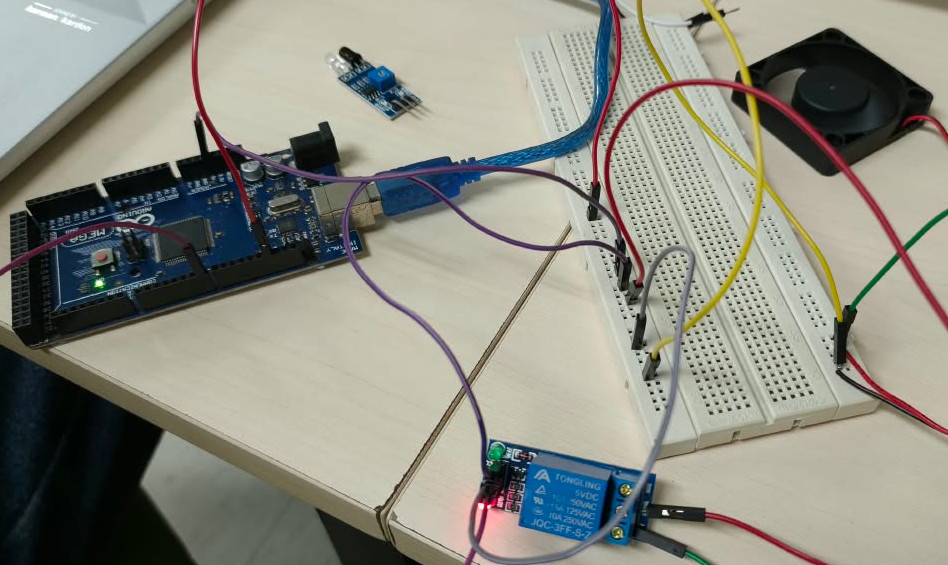
\includegraphics[width=0.55\textwidth]{images/relai_with_fan.jpg}
	\caption{Contoh rangkaian pengontrolan kipas DC menggunakan modul relai.}
	\label{fig:dc_motor_relay_schematic}
\end{figure}

Rincian pemetaan koneksi fisik antara komponen dan fungsi periferal mikrokontroler ATmega2560 dirangkum pada Tabel~\ref{tab:dc_motor_relay_mcu_mapping}.

\begin{table}[H]
	\centering
	\caption{Pemetaan antarmuka pengontrolan Mikro DC Motor 6V via Relai ke Arduino Mega 2560}
	\label{tab:dc_motor_relay_mcu_mapping}
	\small
	\begin{tabularx}{\textwidth}{@{} p{3.5cm} p{3.8cm} X @{}}
		\toprule
		Kebutuhan Komponen   & Fitur MCU                                                        & Alasan Pemilihan \& Fungsi                                                                                                     \\
		\midrule
		Sinyal Pemicu Relai  & Pin GPIO Digital Output 7                                        & Mengirimkan sinyal biner logika LOW/HIGH untuk mengontrol sakelar relai                                                        \\
		Isolasi Daya Kontrol & Optokopler Modul Relai                                           & Memisahkan sirkuit logika $5\,\text{V}$ mikrokontroler dari beban induktif motor $6{,}0\,\text{V}$                             \\
		Catu Daya Utama      & Bus Daya $5\,\text{V}$ MCU \& Sumber $6{,}0\,\text{V}$ Eksternal & Menyediakan daya kumparan relai ($70\,\text{mA}$) dan arus operasional motor DC ($\le 250\,\text{mA}$, maks. $500\,\text{mA}$) \\
		\bottomrule
	\end{tabularx}
\end{table}

\paragraph{Kode Demo Pengujian}
Berikut adalah implementasi program C++ pada Arduino Mega 2560 untuk menguji siklus kerja mati-nyala (\textit{switching}) mikro DC motor 6V melalui modul relai \textit{Active-LOW}:

\begin{lstlisting}[language=C++, caption={Kode program pengontrolan mikro DC motor 6V berbasis modul relai pada Arduino Mega 2560}, label={lst:dc_motor_relay_code}]
#define RELAY_PIN 7

void setup() {
  Serial.begin(9600);
  Serial.println(F("Inisialisasi Pengujian DC Motor via Relai..."));

  pinMode(RELAY_PIN, OUTPUT);
  digitalWrite(RELAY_PIN, HIGH);
}

void loop() {
  Serial.println(F("[STATUS] Mengaktifkan Relai (DC Motor NYALA)"));
  digitalWrite(RELAY_PIN, LOW);
  delay(5000);

  Serial.println(F("[STATUS] Mematikan Relai (DC Motor MATI)"));
  digitalWrite(RELAY_PIN, HIGH);
  delay(3000);
}
\end{lstlisting}

\paragraph{Gambaran Hasil Pembacaan}
Tampilan log keluaran pada \textit{Serial Monitor} saat simulasi pengontrolan DC motor menggunakan modul relai dijalankan adalah sebagai berikut:

\begin{verbatim}
Inisialisasi Pengujian DC Motor via Relai...
[STATUS] Mengaktifkan Relai (DC Motor NYALA)
[STATUS] Mematikan Relai (DC Motor MATI)
[STATUS] Mengaktifkan Relai (DC Motor NYALA)
[STATUS] Mematikan Relai (DC Motor MATI)
\end{verbatim}
